\documentclass{beamer}

\usepackage{graphicx}
\usepackage{hyperref}
\usepackage[latin1]{inputenc}
\usepackage[T1]{fontenc}
\usepackage[english]{babel}
\usepackage{listings}
\usepackage{xcolor,mathrsfs,url}
\usepackage{amssymb}
\usepackage{amsmath}
\usepackage{ifthen}
\usepackage{tikz}
\usepackage{tikz-qtree}
\everymath{\displaystyle}

% The command to define a subsection is '\subsec{}' and NOT '\subsection'.
% This code generates the bar. Don't edit.
\newcommand{\midbarnew}{}
\newcommand{\subsec}[1]
{
  \ifthenelse{\equal{#1}{}}
  {\renewcommand{\midbarnew}{} \subsection{}}
  {\renewcommand{\midbarnew}{ $\mid$ } \subsection{#1}}
}

% change the pictures here, if necessary. logobig and logosmall are the internal names
% for the pictures: do not modify them, just change "hulogo" and "logo". Pictures must be 
% supplied as JPEG, PNG or PDF
%########################################

\pgfdeclareimage[height=2cm]{logobig}{logo} % use hucase instead for the Humboldt-Case Logo
\pgfdeclareimage[height=1cm]{logosmall}{logo}

% use this number to modify the scaling of the headline on titlepage
\def\titlescale{1.0}


\title{Money and Exchange Rates}
\author{Instructor: David Jinkins\thanks{I wish to acknowledge Battista Severgnini for providing last year's slides to me. His generosity saved me much time, and these slides are partially based on his. Any errors are of course my own.}}
\date{Date: Oct. 2, 2014}
%Start of the document
\begin{document}

\frame[plain]{% create the titleslide, layout controlled in metricsbeamer
	\titlepage
}

\frame[plain]{
\frametitle{Last time}
\begin{itemize}
    \item Chapter 13:
    \begin{itemize}
        \item National income accounts
        \item National saving, investment, and the current account
    \end{itemize}
    \item Chapter 14:
    \begin{itemize}
        \item Exchange rate
        \item The foreign exchange market
        \item The demand of currency deposits
        \item Interest rate parity
        \item Partial equilibrium ex. rates
    \end{itemize}
\end{itemize}}

\frame{% how to print
\frametitle{Plan for Today}
\begin{itemize}
    \item Chapter 15
    \begin{itemize}
    \item Money
    \begin{itemize}
        \item What is special about it?
        \item How is it measured?
        \item What determines how much people want?
    \end{itemize}
    \item A Short-run model of the money market
    \item Adjustment in the Long-run
    \begin{itemize}
        \item Why exchange rates are so volatile
    \end{itemize}
    \end{itemize}
    \item Chapter 16
    \begin{itemize}
        \item The law of one price
        \item Purchasing Power Parity
        \item Relative vs. Absolute PPP
    \end{itemize}
    \end{itemize}
}

\begin{frame}{But first a review}
\end{frame}

\frame[plain]{\includegraphics[page=7,width=\textwidth]{national_accounts.pdf}}
\frame[plain]{\includegraphics[page=8,width=\textwidth]{national_accounts.pdf}}
\frame[plain]{\includegraphics[page=9,width=\textwidth]{national_accounts.pdf}}
\frame[plain]{\includegraphics[page=10,width=\textwidth]{national_accounts.pdf}}
\frame[plain]{\includegraphics[page=11,width=\textwidth]{national_accounts.pdf}}
\frame[plain]{\includegraphics[page=13,width=\textwidth]{national_accounts.pdf}}
\frame[plain]{\includegraphics[page=28,width=\textwidth]{national_accounts.pdf}}
\frame[plain]{\includegraphics[page=29,width=\textwidth]{national_accounts.pdf}}
\frame[plain]{\includegraphics[page=30,width=\textwidth]{national_accounts.pdf}}
\frame[plain]{\includegraphics[page=32,width=\textwidth]{national_accounts.pdf}}
\frame[plain]{\includegraphics[page=40,width=\textwidth]{national_accounts.pdf}}
\frame[plain]{\includegraphics[page=41,width=\textwidth]{national_accounts.pdf}}
\frame[plain]{\includegraphics[page=47,width=\textwidth]{national_accounts.pdf}}
\frame[plain]{\includegraphics[page=48,width=\textwidth]{national_accounts.pdf}}
\frame[plain]{\includegraphics[page=53,width=\textwidth]{national_accounts.pdf}}
\frame[plain]{\includegraphics[page=57,width=\textwidth]{national_accounts.pdf}}
\frame[plain]{\includegraphics[page=58,width=\textwidth]{national_accounts.pdf}}
\frame[plain]{\includegraphics[page=59,width=\textwidth]{national_accounts.pdf}}
\frame[plain]{\includegraphics[page=60,width=\textwidth]{national_accounts.pdf}}
\frame[plain]{\includegraphics[page=61,width=\textwidth]{national_accounts.pdf}}
\frame[plain]{\includegraphics[page=65,width=\textwidth]{national_accounts.pdf}}
\frame[plain]{\includegraphics[page=67,width=\textwidth]{national_accounts.pdf}}
\frame[plain]{\includegraphics[page=71,width=\textwidth]{national_accounts.pdf}}
\frame[plain]{\includegraphics[page=72,width=\textwidth]{national_accounts.pdf}}
\frame[plain]{\includegraphics[page=73,width=\textwidth]{national_accounts.pdf}}
\frame[plain]{\includegraphics[page=74,width=\textwidth]{national_accounts.pdf}}

\begin{frame}{Review}
    \begin{itemize}
        \item End review
    \end{itemize}
\end{frame}


\frame{% how to print
\frametitle{}
\begin{center}
\textcolor{blue}{Chapter 15: Money, Interest Rates, and Exchange Rates}
\end{center}
}

\frame{
\frametitle{Money}
\begin{itemize}
    \item Why do we need it?
    \begin{enumerate}
        \item Medium of exchange
        \item Unit of account
        \item Store of value
    \end{enumerate}
\end{itemize}
}

\frame{
\frametitle{Money - Medium of exchange}
\begin{itemize}
    \item Mutual cooincidence of wants
    \begin{itemize}
        \item I want a bottle of water right now
        \item 7-Eleven needs economic analysis right now
    \end{itemize}
    \item Unlikely\dots 
    \item Money helps us:
    \begin{itemize}
        \item Avoid complicated barter exchanges
        \item Automatically get the value of our own production
        \item When we buy something, it is as if we had bartered
    \end{itemize}
\end{itemize}
}

\frame{
\frametitle{Money - unit of account}
\begin{itemize}
    \item Comparing values of different things
    \item Thought experiment
    \begin{itemize}
        \item Suppose that the prices at the canteen in Solberg Plads were all in bananas 
        \item Suppose that the prices at the canteen in Porcelaenshavn were all in toothbrushes 
        \item For ex: Coke costs 10 bananas at SP, and 2 toothbrushes at P
        \item Where is it more expensive?
    \end{itemize}
    \item Money helps us:
    \begin{itemize}
        \item Quickly compare prices across goods and locations
    \end{itemize}
\end{itemize}
}

\frame{
\frametitle{Money - Store of Value}
\begin{itemize}
    \item Money is an asset
    \begin{itemize}
        \item If you want, keep in under your mattress!
    \end{itemize}
    \item It is the most liquid asset, a benchmark
\end{itemize}
}

\frame{
\frametitle{What is money?}
\begin{itemize}
    \item More difficult question than it seems!
\end{itemize}
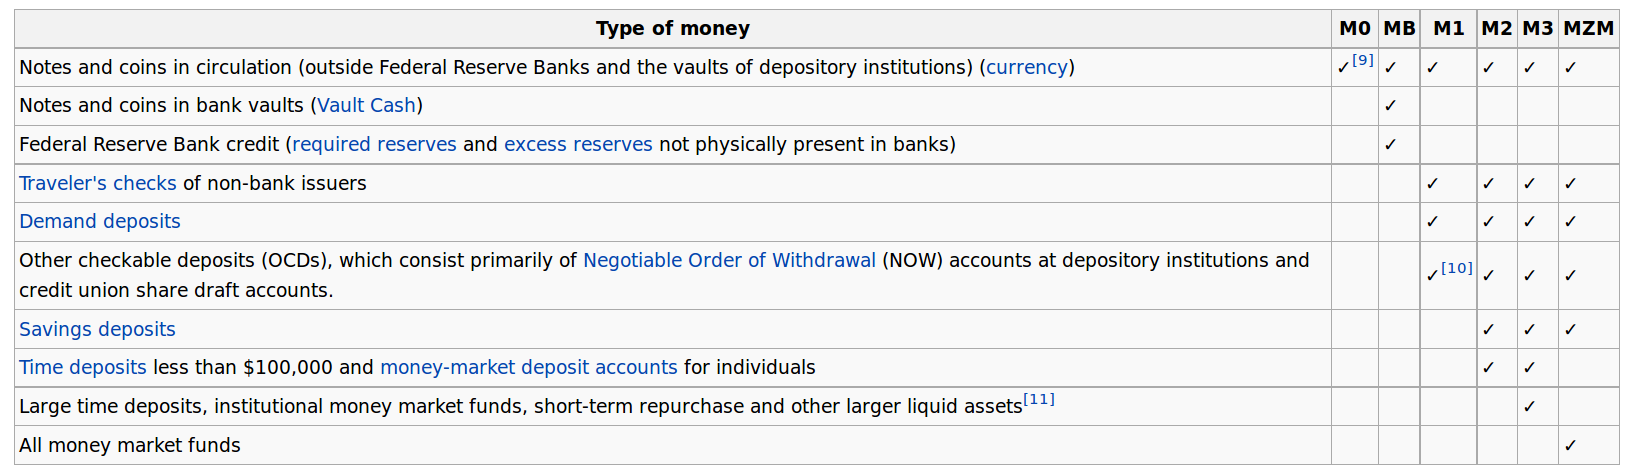
\includegraphics[scale=0.20]{money_supply.png}
\begin{itemize}
    \item M1 is the most liquid
    \item In this book, \emph{money supply} is M1
\end{itemize}
}

\frame{
\frametitle{A difficult quesiton}
\begin{itemize}
    \item Money does three things
    \begin{enumerate}
        \item Medium of exchange
        \item Unit of account
        \item Store of value
    \end{enumerate}
    \item Why do we use pieces of paper and not gold coins?
    \item Or at least pieces of paper that could be redeemed for gold 
    \begin{itemize}
        \item What is the advantage we get from paper?
        \item Gold has an advantage: independent value\dots
    \end{itemize}
    \item Bitcoin\dots
\end{itemize}
}

\frame{
\frametitle{Money Supply \& Demand}
\begin{itemize}
\item \textbf{money supply} controlled by Central Bank 
\begin{itemize}
    \item Actually process a bit complicated, see Chpt. 18
    \item For now just assume M1 chosen by Central Bank
\end{itemize}
\item \textbf{money demand} represents the amount of monetary assets that people are willing to hold. This is based on:
\begin{enumerate}
\item Interest rates/expected rates of return 
\item Risk/inflation
\item Liquidity
\end{enumerate}
\end{itemize}
}

\frame{
\frametitle{Expected return and interest}
\begin{itemize}
    \item M1 pays no interest (to a first approximation)
    \item If hold cash, lose interest gained by holding illiquid asset
    \item The higher the interest rate, the higher opportunity cost of holding cash
    \begin{itemize}
        \item One safe way of earning interest is a risk-free bond
        \item Classic example, American T-Bill
        \item The higher the return on T-Bill, the less demand for cash
    \end{itemize}
\end{itemize}
}

\frame{
\frametitle{Risk}
\begin{itemize}
    \item Textbook claims risk is not important
    \item Argument, all financial assets are denoted in currency
    \item Can't insure against risk
    \item I'm not sold on this argument: flexible rate bonds, bonds denoted in gold, etc
    \item OK as a first approximation
\end{itemize}
}

\frame{
\frametitle{Liquidity}
\begin{itemize}
    \item Main use of cash -- financing everyday purchases 
    \item More purchases you make, the more cash you need
    \item Debit card (Dankort) purchases still in M1
    \item Credit card purchases also involve cash transfers
\end{itemize}
}

\frame{
\frametitle{Individual demand for money}
\begin{itemize}
    \item Decreasing in the interest rate on other assets
    \item Mostly unrelated to risk
    \item Increasing in the amount of daily purchases
\end{itemize}
}

\frame{
\frametitle{Aggregate Money Demand}
\begin{itemize}
    \item Sum up all individual demand
    \item The aggregate demand of real money can be expressed as:
\end{itemize}
\begin{center}
$\frac{M^{d}} =P L\left(R,Y\right)$
\end{center}
where:
\begin{itemize}
\item $P$ is the price level: higher prices, more cash needed
\item $Y$ is real national income: more stuff, more purchases
\item $R$ is a measure of interest rates on non-monetary assets
\item $L\left(R,Y\right)$ is the aggregate demand of real monetary assets
\end{itemize}
}

\frame{
\frametitle{Aggregate Demand of Real Money}
\begin{center}
$\frac{M^{d}}{P} =L\left(R,Y\right)$
\end{center}
\begin{itemize}
\item $M^{d}$ scales perfectly with $P$
\item If all prices double, need twice as much cash
\item Demand for real money
\end{itemize}
\begin{center}
$\frac{M^{d}}{P} =L\left(R,Y\right)$
\end{center}
\begin{itemize}
    \item The L function is demand for holding real value in liquid form
\end{itemize}
}

\begin{frame}{Money demand and interest rate}
    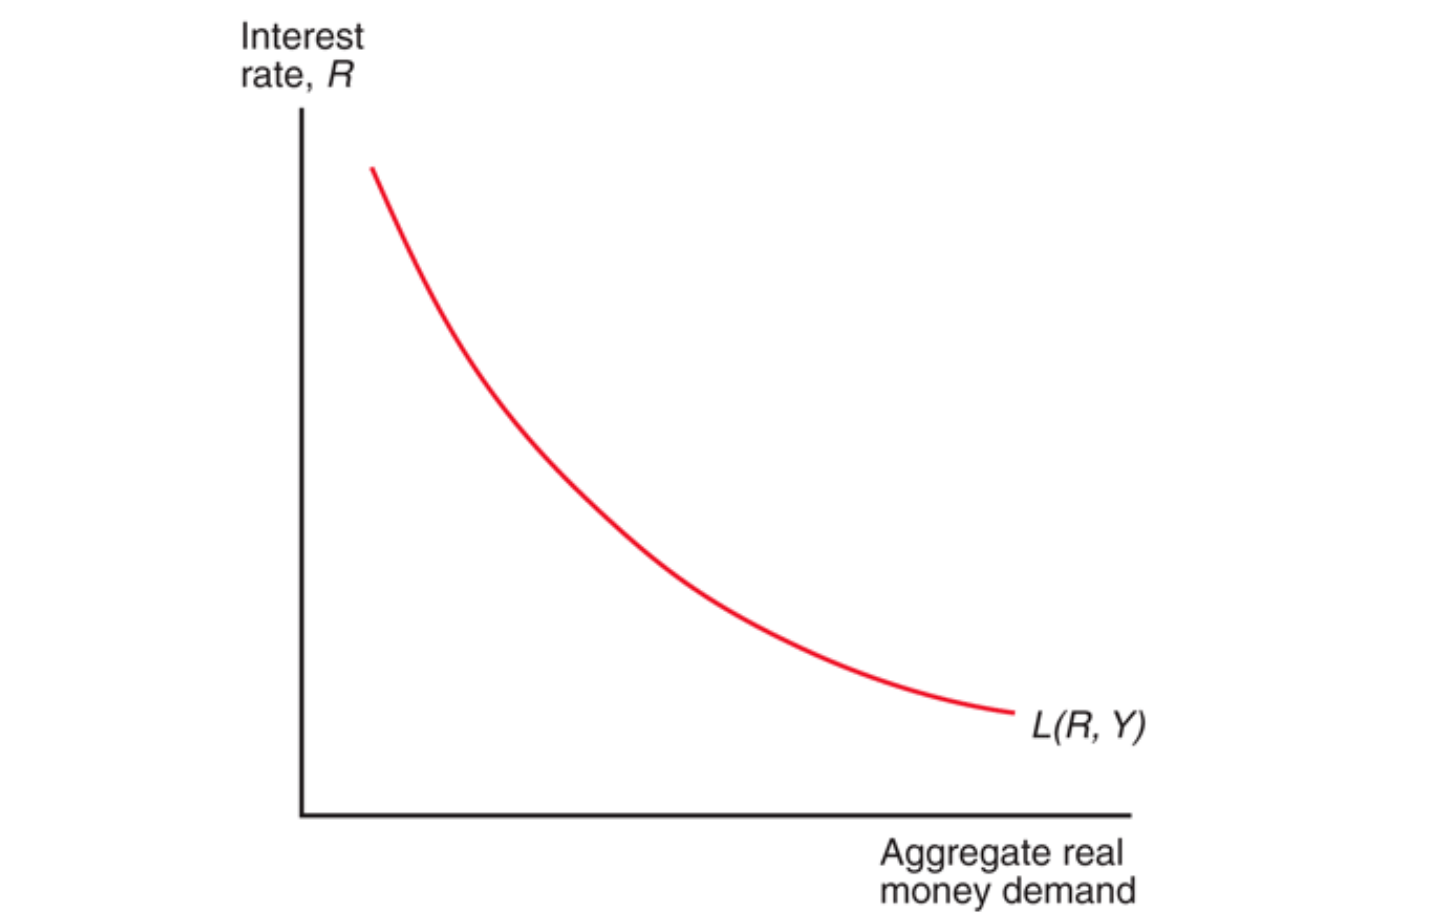
\includegraphics[scale=.25]{int_demand.png}
\end{frame}

\begin{frame}{Shift in National Product}
    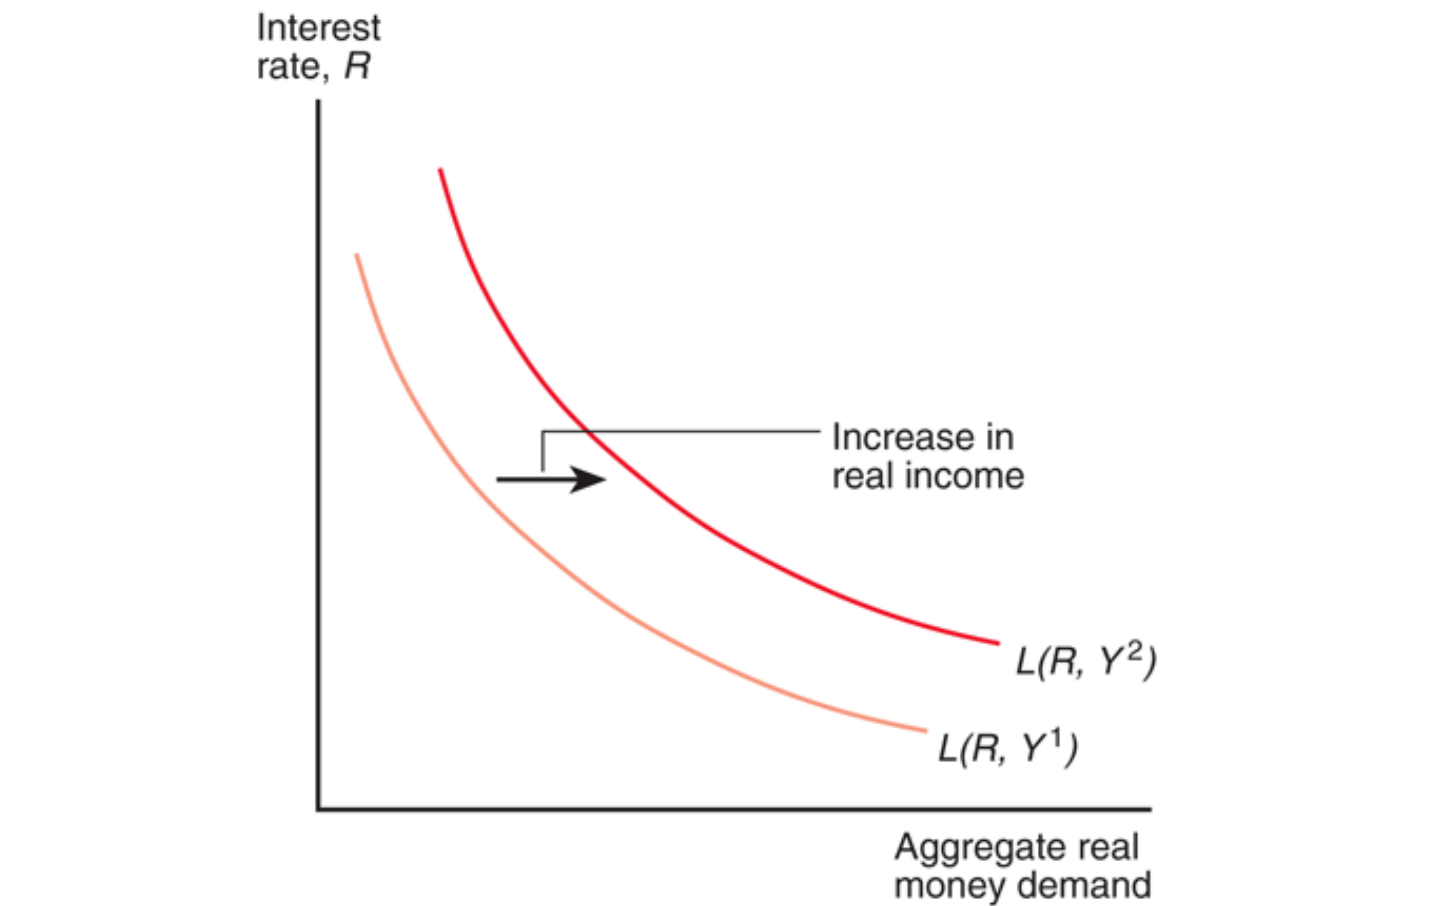
\includegraphics[scale=.25]{GNP_shift.png}
\end{frame}

\frame{
\frametitle{A Short-run Model of the Money Market}
\begin{itemize}
    \item Assume that changes in money supply do not affect:
    \begin{enumerate}
        \item Price level
        \item GNP level
    \end{enumerate}
    \item Changes do affect interest rate of other assets
    \item In equilibrium:
\begin{center}
$M^{s}=M^{d}$
\end{center}
\item Plug in our formula for money demand, in equilibrium
\begin{center}
$\frac{M^{s}}{P} =L\left(R,Y\right)$
\end{center}
\item Real money supply (LHS) equals real money demand (RHS)
\item Higher money supply $\Rightarrow$ lower interest rate
\end{itemize}
}

\frame{
\frametitle{Money supply and interest rate in the short-run}
\begin{itemize}
    \item If more supply than demand for money:
    \begin{enumerate}
        \item People with money will buy bonds for lower interest rate
        \item As interest rates fall, people more willing to hold money
    \end{enumerate}
    \item If more demand than supply for money:
    \begin{enumerate}
        \item People will promise more money in the future for money today 
        \item As interst rates rise, people less willing to hold money
    \end{enumerate}
\end{itemize}
}

\frame{
\frametitle{Determination of the Equilibrium Interest Rate}
\begin{figure}
	\centering
		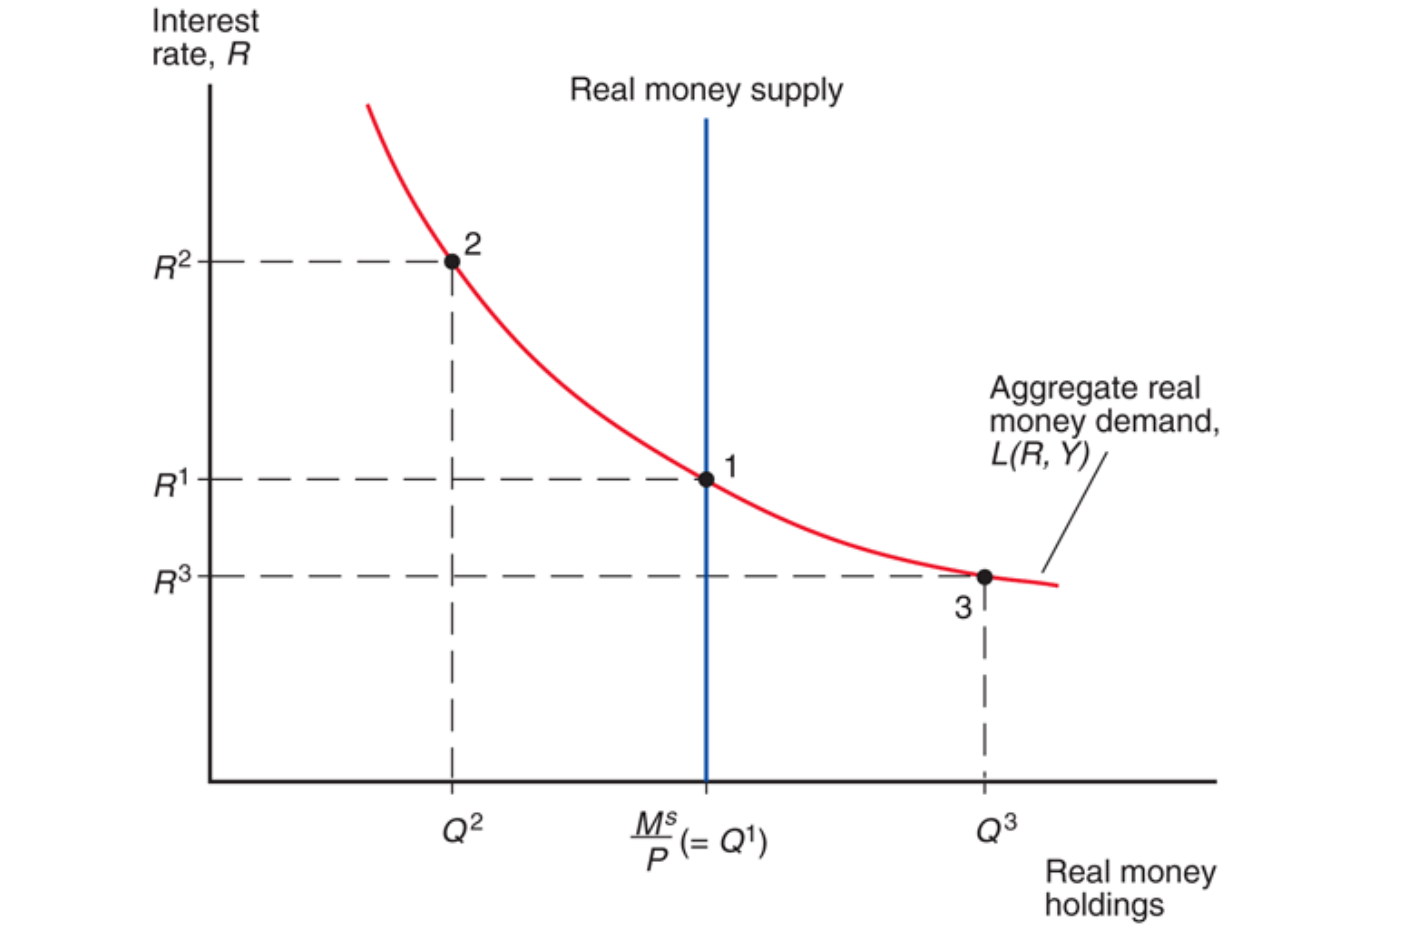
\includegraphics[scale=0.25]{supply_demand.png}
\end{figure}
}

\frame{
\frametitle{Effect of an Increase in the Money Supply on the Interest Rate}
\begin{figure}
	\centering
		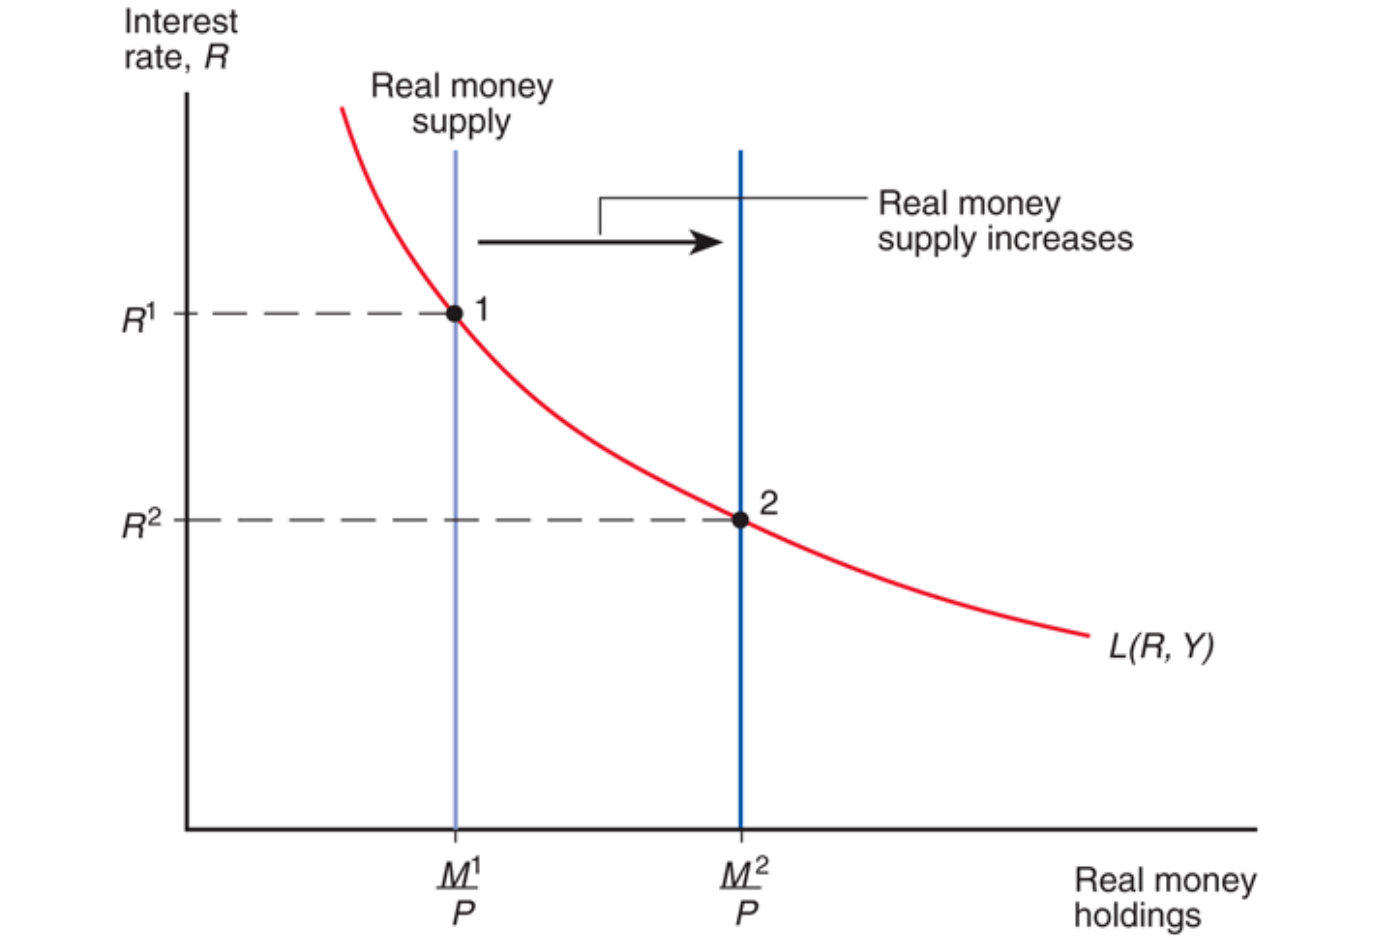
\includegraphics[scale=0.15]{supply_interest.png}
	\label{fig:11}
\end{figure}
\begin{itemize}
    \item Short run: Central bank can lower interest rate by increasing money supply
    \item Short run: Central bank can raise interest rate by decreasing money supply
\end{itemize}
}


\frame{
\frametitle{Effect on the Interest Rate of a Rise in Real Income}
\begin{figure}
	\centering
		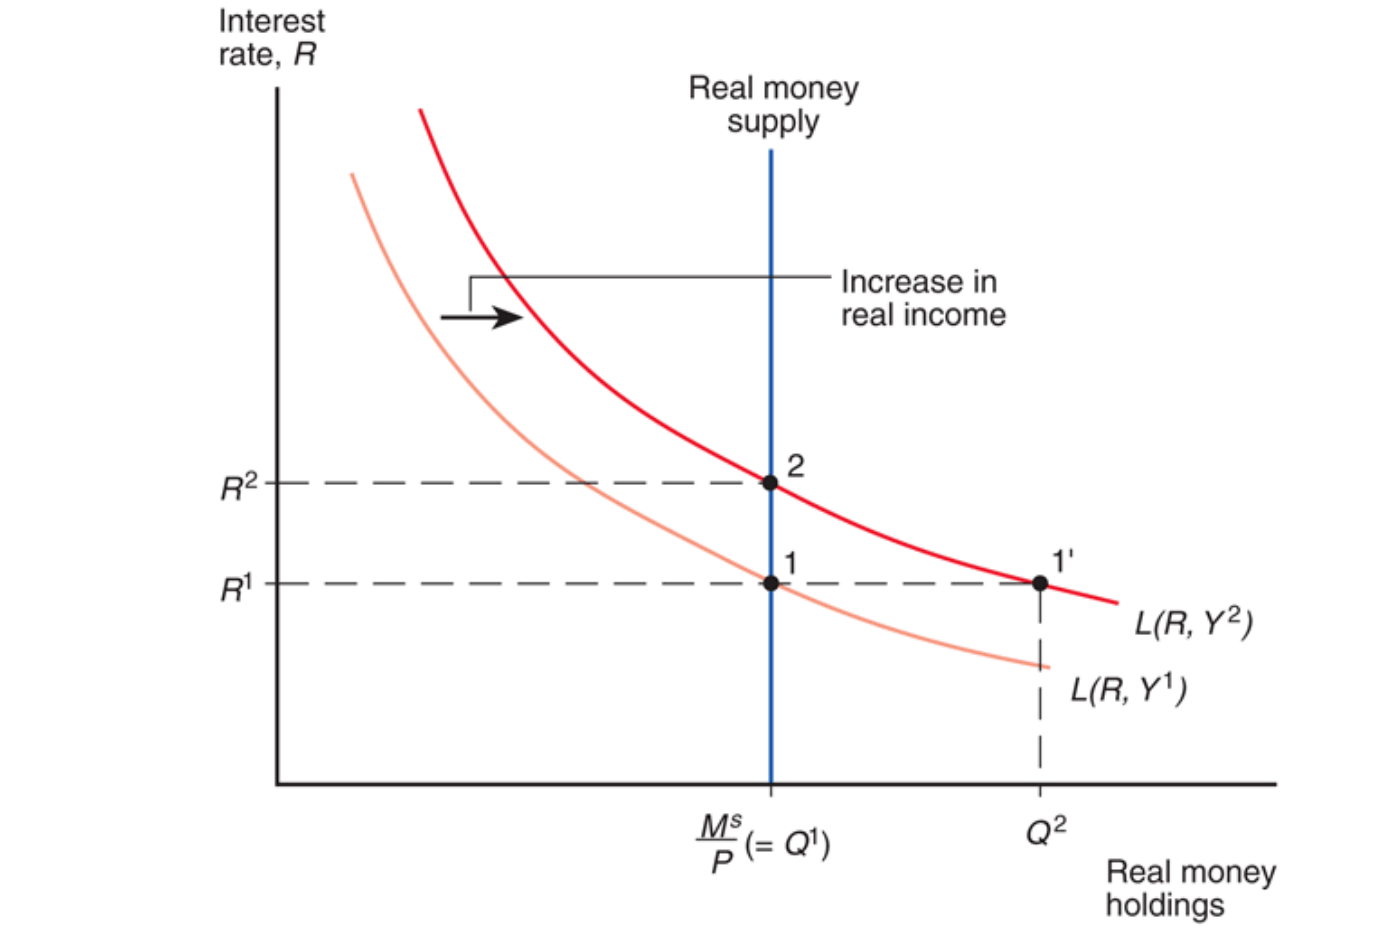
\includegraphics[scale=0.20]{supply_real_income.png}
\end{figure}
\begin{itemize}
    \item Short run: Output growth increases interest rate
    \item Short run: A fall in output decreases interest rate
\end{itemize}
}

\begin{frame}{Reminder: Interest rate parity condition}

    \begin{itemize}
        \item Assume that the return on Euro bonds is fixed in Euros
        \item Given dollar interest rate, exchange rate adjusts to satisfy parity 
    \end{itemize}
		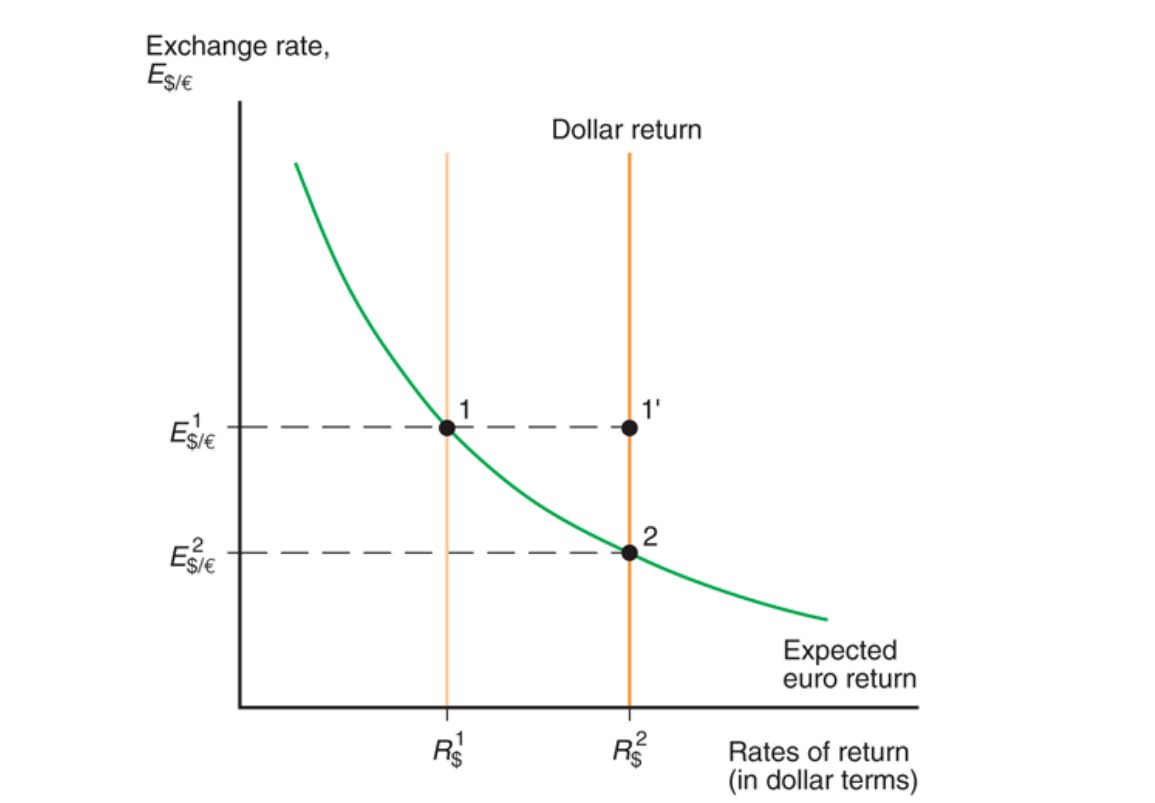
\includegraphics[scale=0.20]{interest_rate_parity.png}
\end{frame}

\begin{frame}{Money supply and exchange rate}

    \begin{itemize}
        \item Suppose Central Bank ups money supply
        \item Interest rate goes down as people buy bonds
        \item Dollar depreciates to maintain interest parity 
    \end{itemize}
\end{frame}

\frame{
\frametitle{Money supply and exchange rate}
\begin{figure}
	\centering
		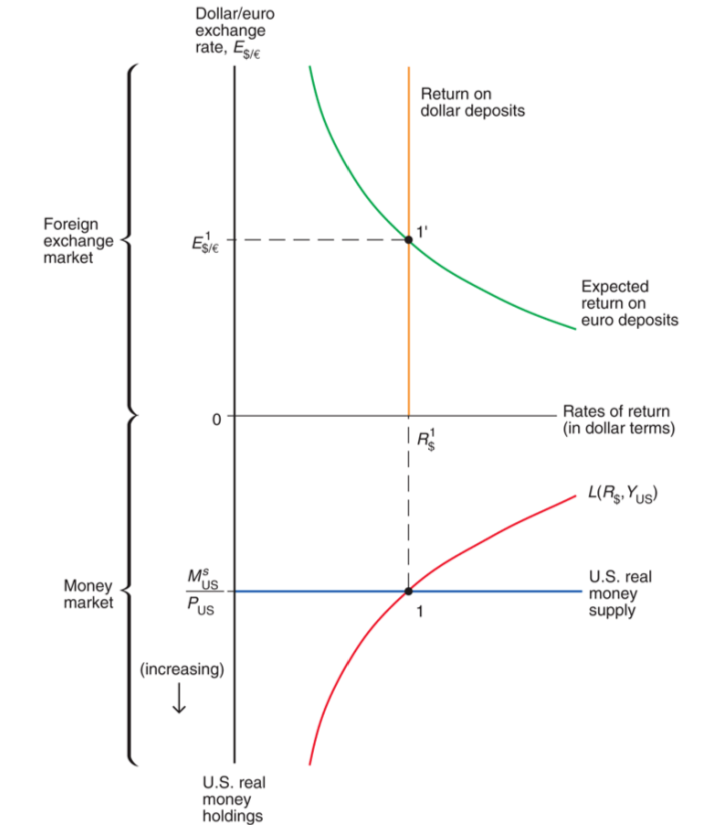
\includegraphics[scale=0.28]{money_exchange.png}
\end{figure}
}

\frame{
\frametitle{Money Market/Exchange Rate Linkages}
    \begin{itemize}
        \item It is a two central bank game! 
    \end{itemize}
\begin{figure}
	\centering
		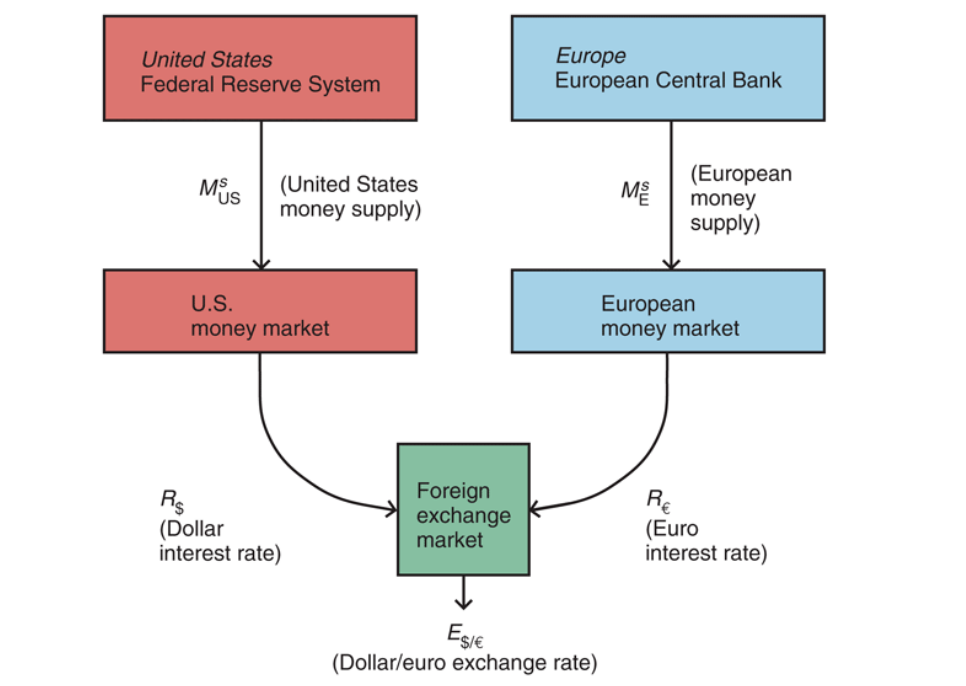
\includegraphics[scale=0.28]{dollar_euro.png}
\end{figure}
}

\frame{
\frametitle{Increase in dollar supply}
\begin{figure}
	\centering
		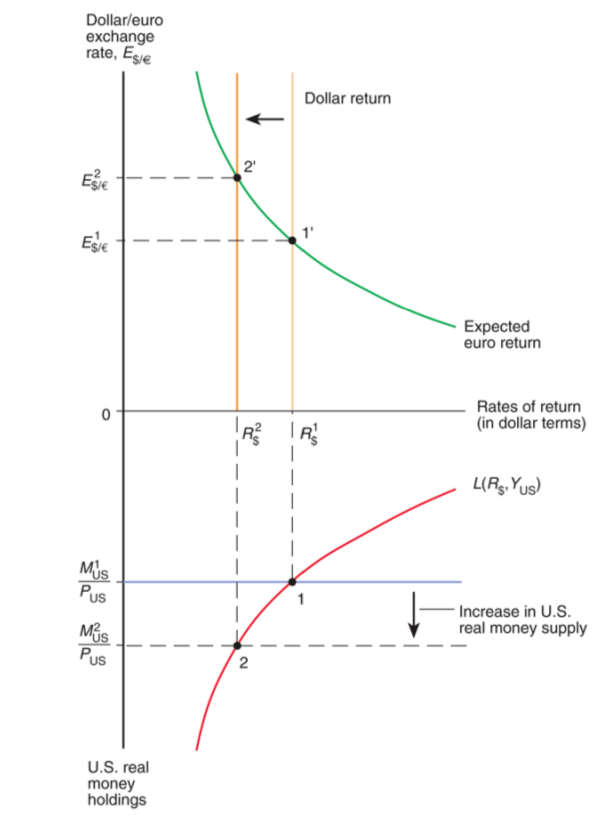
\includegraphics[scale=0.28]{dollar_increase.png}
\end{figure}
}

\frame{
\frametitle{Increase in euro supply}
\begin{figure}
	\centering
		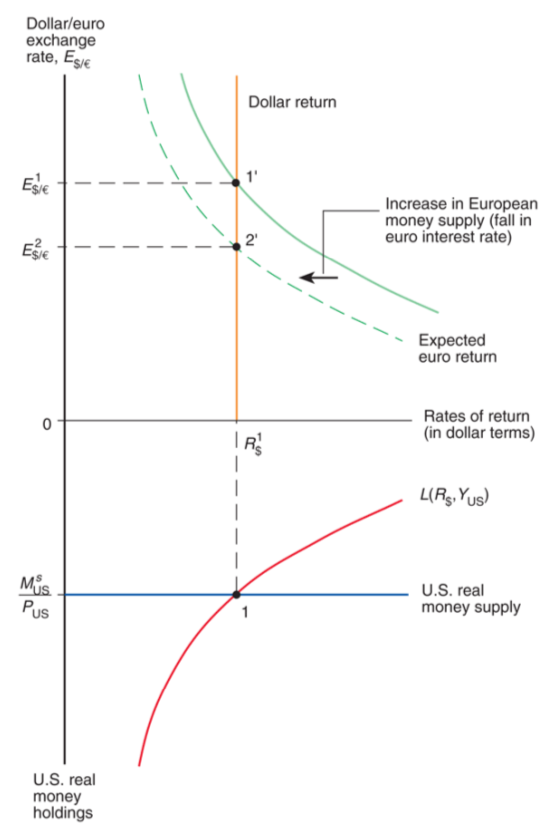
\includegraphics[scale=0.28]{euro_increase.png}
\end{figure}
}



\frame{
\frametitle{Changes in the Domestic Money Supply}
An increase in a country's money supply:
\begin{itemize}
\item $R \Downarrow$
\item depreciation of the domestic currency
\end{itemize}
An decrease in a country's money supply:
\begin{itemize}
\item $R \Uparrow$
\item appreciation of the domestic currency
\end{itemize}
}


\frame{
\frametitle{Changes in the Foreign Money Supply}
How would a change in the supply of euros  affect the U.S. money market and foreign exchange markets?
\begin{itemize}
\item An increase in the supply of euros $\Rightarrow$ depreciation of the euro
\begin{enumerate}
    \item $R_{EURO} \Downarrow$
\item depreciation of the euro
\end{enumerate}
\item A decrease in the supply of euros $\Rightarrow$ appreciation of the euro
\end{itemize}
}

\frame{
\frametitle{Long \& Short Run}
\begin{itemize}
    \item Affect of more money supply
    \item \textbf{Short run:} Prices are sticky, real money supply rises
    \item \textbf{Long run:} Prices adjust so that real money supply falls to its original level
\end{itemize}
}

\frame{
\frametitle{In the Long Run}
In the long run, there is a direct relationship between the inflation rate and changes in the money supply.
\begin{itemize}
\item $M^{s} = P  L\left(R,Y\right)$
\item $P =\frac{M^{s}}{L\left(R,Y\right)}$
\end{itemize}
Money supply has no long run effecton output and interest rates
% \item $\frac{\Delta P}{P} = \frac{\Delta M^{s}}{M^{s}} - \frac{\Delta L}{L}$
% \end{itemize}
% The inflation rate is predicted to equal the growth rate in money supply minus the growth rate in money demand.
}

\frame{
\frametitle{Money supply, output and interest}
\begin{itemize}
\item Money supply has no long run effecton output and interest rates
\item Intuition
\begin{itemize}
    \item A currency reform: Turkish millionaires
    \item 2005, new Turkish lira, divide old lira by one million
    \item For a period, both lira could be used
    \item Everything in the country lost six zeros
    \item No effect on output or interest
\end{itemize}
\item Central Bank actions are similar
\item Double the money, halve the prices
\end{itemize}
}

\frame{
\frametitle{Money supply, demand, and inflation}
\begin{itemize}
    \item Long run prices:
    \item $P =\frac{M^{s}}{L\left(R,Y\right)}$
    \item $\frac{\Delta P}{P} = \frac{\Delta M^{s}}{M^{s}} - \frac{\Delta L}{L}$
\end{itemize}
The inflation is the growth rate in money supply minus the growth rate in money demand.
}

\frame[plain]{
\frametitle{Average Money Growth and Inflation in Western Hemisphere Developing Countries, by Year, 1987-2007}
\begin{figure}
	\centering
		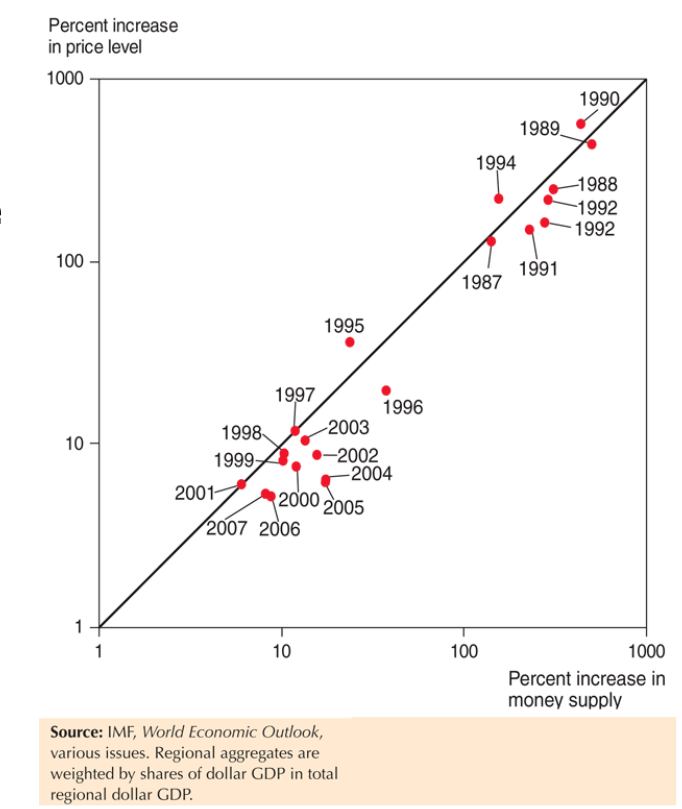
\includegraphics[scale=0.28]{inflation_supply.png}
	\label{fig:11}
\end{figure}
}

\frame{
\frametitle{Short run and Long run}
\begin{itemize}
    \item Money cannot shift prices immediately
    \begin{itemize}
        \item Long-term contracts
        \item Menu costs
    \end{itemize}
\end{itemize}
}

\begin{frame}{Exchange Rates vs Price Level}
\begin{itemize}
    \item In short-run example, we let exchange rates adjust, not prices;
    \item This assumption seems reasonable for US and Japan
\end{itemize}
		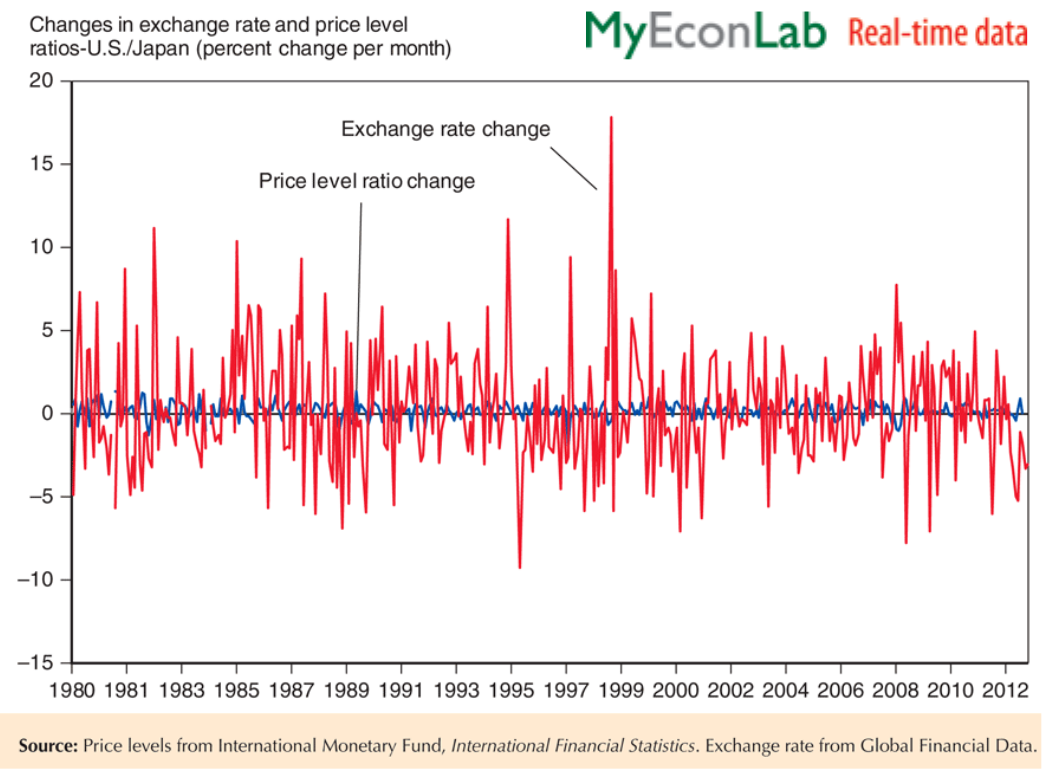
\includegraphics[scale=0.28]{us_japan_prices.png}
\end{frame}

\frame{
\frametitle{Short run and Long run}
\begin{itemize}
    \item Money cannot shift prices immediately
    \item Over time, however, prices will adjust
    \begin{enumerate}
    \item Excess demand of goods and services: labor $\Uparrow$ $\Rightarrow$ wage $w \Uparrow$  $ P \Uparrow$
    \item Inflationary expectations: $P^{e} \Uparrow w \Uparrow P \Uparrow$
    \item Raw materials prices: Adjust quickly
    \end{enumerate}
\end{itemize}
}

\frame[plain]{
\frametitle{Excess demand for factors}
\begin{itemize}
    \item More money but the same prices means people buy more
    \item To produce more, firms have to buy more inputs
    \item Old workers are stuck on contract
    \item New workers can bargain for higher wages
    \item The increase in input price causes increase in output price
\end{itemize}
}

\frame[plain]{
\frametitle{Inflationary expectations}
\begin{itemize}
    \item People know about increse in money supply 
    \item Long run, prices will rise
    \item Workers bargaining for Long-term contracts will demand higher wages
\end{itemize}
}

\frame[plain]{
\frametitle{Raw materials}
\begin{itemize}
    \item The price of raw materials (oil) adjusts quickly
    \item Output prices eventually need to reflect increase in input cost
\end{itemize}
}

\begin{frame}{Money supply and exchange rates, long-run}
\begin{itemize}
    \item Review: 
    \begin{itemize}
        \item The return to Euro bonds in dollars depends on expected depreciation
        \item The more the dollar is expected to depreciate, the higher Euro bond returns
    \end{itemize}
    \item Permanent money supply increases raise expected depreciation
\end{itemize}
\end{frame}

\begin{frame}{Money supply and exchange rates, long-run}
\begin{itemize}
    \item Review: 
    \begin{itemize}
        \item The return to Euro bonds in dollars depends on expected depreciation
        \item The more the dollar is expected to depreciate, the higher Euro bond returns
    \end{itemize}
    \item Permanent money supply increases raise expected depreciation
\end{itemize}
\end{frame}

\begin{frame}{Increase in money supply and exchange rate, long-run}
\begin{itemize}
    \item Initially:
    \begin{itemize}
        \item Money supply goes up, interest rate falls, depreciation
        \item Money supply goes up, expected depreciation, more depreciation
    \end{itemize}
    \item Then:
    \begin{itemize}
        \item Prices adjust to long run real money supply level
        \item Real money supply falls, interest rate rises, appreciation
        \item Exchange rate settles level depreciated relative to initial level
    \end{itemize}
    \item The double depreciation followed by appreciation: \emph{exchange rate overshoot}
\end{itemize}
\end{frame}

\frame{
\frametitle{Money, Prices, Exchange Rates, and Expectations}
\begin{figure}
	\centering
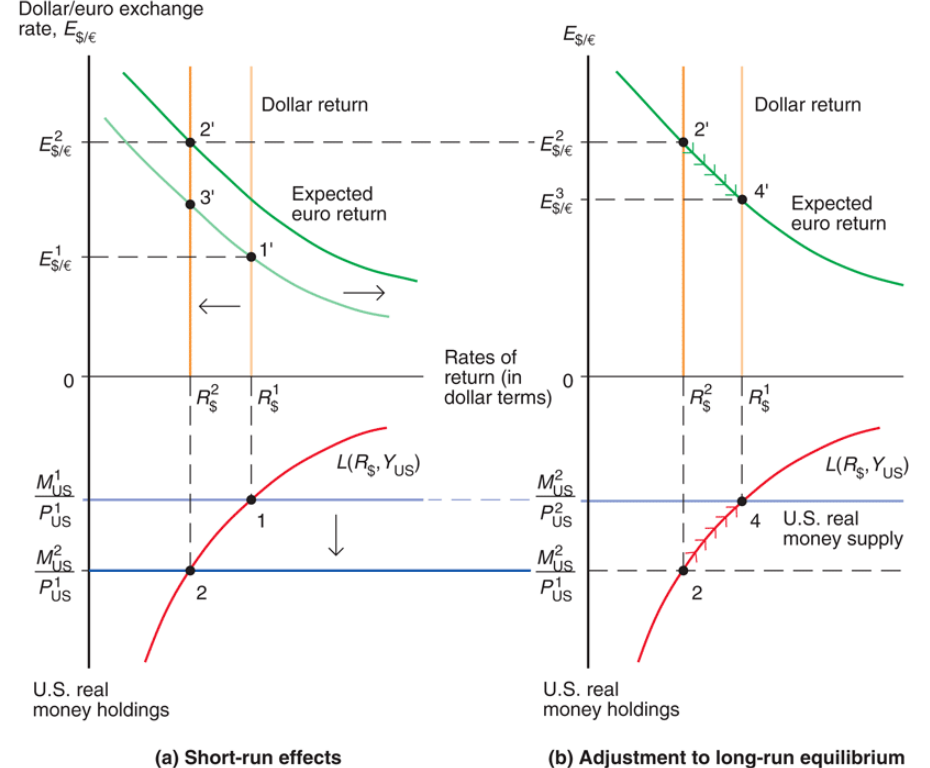
\includegraphics[scale=0.25]{long_run_exchange.png}
\end{figure}
}

\frame[plain]{
\frametitle{Money, Prices, Exchange Rates, and Expectations}
\begin{figure}
	\centering
    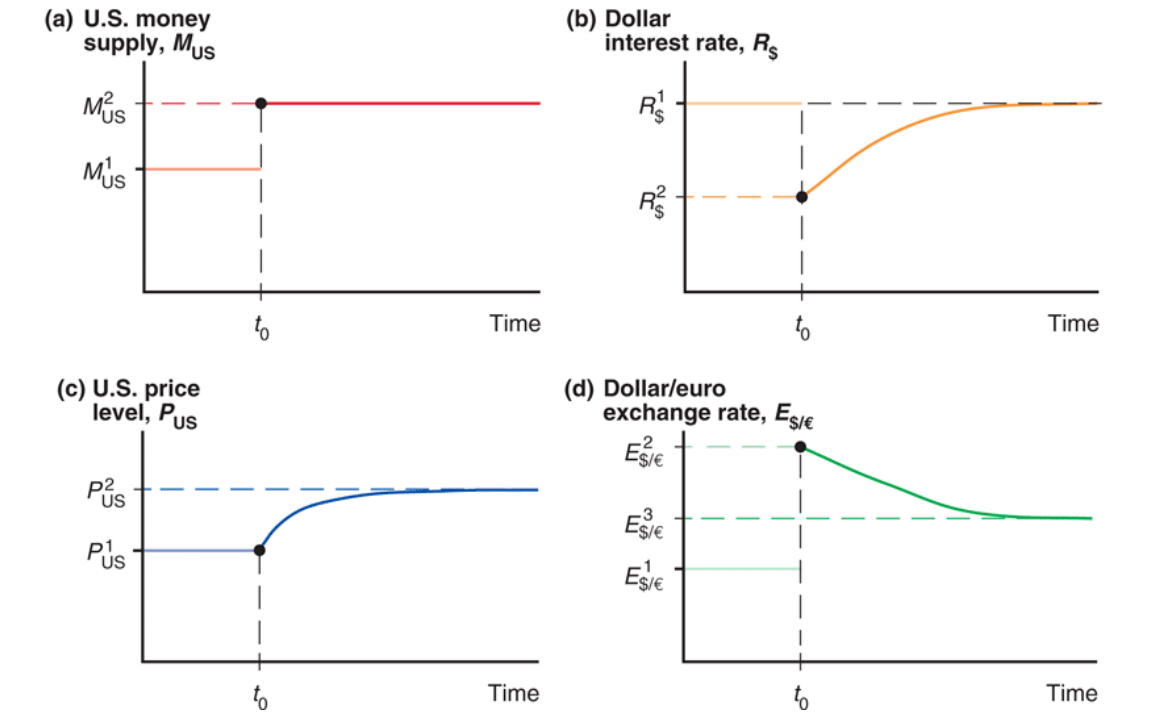
\includegraphics[scale=0.25]{macro_impulse.png}
	\label{fig:11}
\end{figure}
}

\begin{frame}{Summary of Chapter 15}
    \begin{itemize}
        \item We have seen short run sticky prices which cause short-run real effects
        \item We have seen that in the long run, money is neutral (no real affect)
        \item We have seen that expectations about money supply affect current exchange rates
        \item In Chapter 16, we will study how long-term demand and supply shifts affect exchange rate
        \item Discussion builds on the linkages studied in Chapter 15
    \end{itemize}
\end{frame}

\frame{% how to print
\frametitle{}
\begin{center}
\textcolor{blue}{Chapter 16: Price Levels and the Exchange Rate in the Long Run
}
\end{center}
}


\frame{
\frametitle{The Law of One Price (1)}
The prices of identical goods sold in different
countries must be the same when expressed
in terms of the same currency.
\begin{itemize}
\item  This law applies only in competitive markets
free of transport costs and official barriers to
trade.
\item Example: If the dollar/pound exchange rate
is USD 1.50 per pound, a sweater that sells for
USD 45 in New York must sell for �30 in London.
\end{itemize}
}


\frame{
\frametitle{The Law of One Price (2)}
The dollar price of good i is the same wherever it
is sold
\begin{center}
$P^{i}_{US} = \left(E_{USD/EURO}\right) x \left(P^{i}_{E}\right)$
\end{center}
where:
\begin{itemize}
\item $P^{i}_{US}$ is the dollar price of good i when sold in
the U.S.
\item $P^{i}_{EURO}$ is the corresponding euro price in Europe
\item $\left(E_{USD/EURO}\right)$ is the dollar/euro exchange rate
\end{itemize}}

\frame{
\frametitle{Purchasing Power Parity  (PPP)(1)}
PPP 
\begin{itemize}
\item is the application of the law of one price across countries for \textit{all} goods and services.
\item compares average prices across countries
\item predicts a dollar/euro exchange rate of
\begin{center}
$ E_{USD/EURO} =\frac{P_{US}}{P_{E}}$
\end{center}
where
\begin{itemize}
\item $P_{US}$ is the dollar price of a reference commodity
basket sold in the United States
\item $P_{E}$ is the euro price of the same basket in Europe
\end{itemize}
\end{itemize}
}

\frame{
\frametitle{Purchasing Power Parity (PPP)(2)}
Rearranging,
\begin{center}
$ P_{US}=\left(E_{USD/EURO}\right)x\left(P_{E}\right)$
\end{center}
All countries' price levels are equal when measured in
terms of the same currency
}

\frame{
\frametitle{PPP \& Law of One Price}
\begin{itemize}
\item The law of one price applies to individual
commodities; PPP applies to the general
price level
\item If the law of one price holds true for every
commodity $\Rightarrow$ PPP must hold for the same
reference baskets across countries
\item BUT if PPP holds, this does not mean that law of one price is respected
\end{itemize}
}


\frame{
\frametitle{Purchasing Power Parity (PPP)(3)}
\begin{enumerate}
\item Absolute PPP: exchange rates equal relative price levels
\item Relative PPP: the percentage change in the exchange
rate between two currencies equals the difference
between the percentage changes in national price
levels.
\begin{center}
$\frac{\left(E_{USD/EURO,t} - E_{USD/EURO,t}\right)}{ E_{USD/EURO,t-1}}= \pi_{US, t} - \pi_{EUROPE, t}$
\end{center}
\end{enumerate}
where $\pi_{t}$ = inflation rate from period $t-1$ to $t$
}


\frame{
\frametitle{Absolute \& Relative PPP (1)}
If absolute PPP holds $\Rightarrow$ relative PPP holds
\begin{table}
\begin{center}
\begin{tabular}{||c|c|c||}\hline
 & $t$ & $t+1$ \\\hline
Absolute & $P_{US,t-1}=USD 100$ & $P_{US,t-1}= USD110$ \\ 
PPP      & $E_{t-1}P_{EURO,t-1}=USD100$ & $E_{t}P_{EURO,t} = USD110$ \\ \hline
\multicolumn{3}{||c||}{$\Rightarrow$} \\ \hline
Relative & \multicolumn{2}{|c||}{$\pi_{US, t}=10\%$}\\
PPP      & \multicolumn{2}{|c||}{$\pi_{EUROPE, t}=\frac{\left(E_{t} - E_{t-1}\right)}{ E_{t-1}}$}\\\hline \hline
\end{tabular}
\end{center}
\end{table}
}


\frame{
\frametitle{Absolute \& Relative PPP (2)}
\textbf{Not the other way around!}
\begin{table}
\begin{center}
\begin{tabular}{||c|c|c||}\hline
 & $t$ & $t+1$ \\\hline
Relative & \multicolumn{2}{|c||}{$\pi_{US, t}=10\%$}\\
PPP      & \multicolumn{2}{|c||}{$\pi_{EUROPE, t}=\frac{\left(E_{t} - E_{t-1}\right)}{ E_{t-1}}$} \\\hline
\multicolumn{3}{||c||}{NOT TRUE $\Rightarrow$} \\ \hline
Absolute & $P_{US,t-1}=USD 200$ & $P_{US,t-1}= USD220$ \\ 
PPP      & $E_{t-1}P_{EURO,t-1}=USD100$ & $E_{t}P_{EURO,t} = USD110$ \\ \hline \hline
\end{tabular}
\end{center}
\end{table}
}

\begin{frame}
    \begin{itemize}
        \item Next time we will continue our discussion of Chapter 16
    \end{itemize}
\end{frame}

\frame{
\frametitle{A Long-Run Exchange Rate
Model Based on PPP}
\begin{itemize}
\item Monetary approach to the exchange rate
\item A theory of how exchange rates and
monetary factors interact in the long run.
\item The fundamental equation of the monetary
approach
\item Price levels can be expressed in terms of
domestic money demand and supplies.
\end{itemize}
\begin{enumerate}
\item In the United States:
\begin{center}
$P_{US}= \frac{M^{s}_{US}}{L \left(R_{USD}, Y_{US}\right)}$
\end{center}
\item In Europe:
\begin{center}
$P_{EUROPE}= \frac{M^{s}_{EURO}}{L \left(R_{EURO}, Y_{EUROPE}\right)}$
\end{center}
\end{enumerate}}


\frame{
\frametitle{PPP and Money Market}
\begin{center}
$E=\frac{P_{US}}{P_{EURO}}=\frac{\frac{M^{s}_{US}}{L \left(R_{USD}, Y_{US}\right)}}{\frac{M^{s}_{EURO}}{L \left(R_{EURO}, Y_{EUROPE}\right)}}$
\end{center}
Specific Predictions:
\begin{enumerate}
\item Money supplies: if $M^{s}_{US} \left(M^{s}_{EU}\right) \Uparrow \Rightarrow$ long-run depreciation (appreciation) of the dollar against the euro
\item interest rates: if $R_{USD} \left(R_{EU}\right) \Uparrow \Rightarrow$  
causes a depreciation (appreciation) of the dollar against the
euro
\item Output levels: a rise if $Y_{US} \left(Y_{EUROPE}\right) \Uparrow \Rightarrow$ causes an appreciation
(depreciation) of the dollar against the euro.
\end{enumerate}
}



\frame{
\frametitle{The Fisher Effect (1)}
\begin{itemize}
\item A more reasonable description of
monetary policy is constantly growing
money supply
\item Money supply grows at a constant
growth rate results in ongoing inflation
at the same rate
\end{itemize}
}

\frame{
\frametitle{The Fisher Effect (2)}
\begin{center}
$E=\frac{P_{US}}{P_{EURO}}=\frac{\frac{M^{s}_{US}}{L \left(R_{USD}, Y_{US}\right)}}{\frac{M^{s}_{EURO}}{L \left(R_{EURO}, Y_{EUROPE}\right)}}$
\end{center}
Given $M^{s}_{EURO}$ and $P_{EURO}$ constant, if $M^{s}_{US}$ grows by $\pi$, $P_{US}$ grows by $\pi$
\begin{center}
$\Rightarrow$
\end{center}
\begin{center}
$E$ depreciated by $\pi$ each period
\end{center}
\begin{center}
$\frac{E_{t}-E_{t-1}}{E_{t}}=\pi_{t}-\pi_{t-1}$
\end{center}
Monetary policies in
the US and Euroland determine the
development in the exchange rate
}


\frame[plain]{
\frametitle{The Fisher Effect (3)}
Given Uncovered Interest Rate Parity,
\begin{center}
$R_{USD,t}= R_{EURO,t}+\left(\frac{E^{e}_{EURO,USD,t+1}-E_{EURO,USD,t}}{E_{EURO,USD,t}}\right)$
\end{center}
and relative PPP
\begin{center}
$\frac{\left(E_{USD/EURO,t} - E_{USD/EURO,t}\right)}{ E_{USD/EURO,t-1}}= \pi_{US, t} - \pi_{EUROPE, t}$
\end{center}
\begin{center}
$\Rightarrow$
\end{center}
Real interest rates are equal
\begin{center}
$\Rightarrow$
\end{center}
\begin{center}
$R_{USD} - R_{EURO} = \pi^{e}_{US} - \pi^{e}_{EUROPE}$
\end{center}
or
\begin{center}
$R_{USD} - \pi^{e}_{US} = R_{EURO}- \pi^{e}_{EUROPE}$
\end{center}
}


\frame{
\frametitle{The Fisher Effect (4)}
Given Uncovered Interest Rate Parity,
\begin{center}
$R_{USD,t}= R_{EURO,t}+\left(\frac{E^{e}_{EURO,USD,t+1}-E_{EURO,USD,t}}{E_{EURO,USD,t}}\right)$
\end{center}
and relative PPP
\begin{center}
$\frac{\left(E_{USD/EURO,t} - E_{USD/EURO,t}\right)}{ E_{USD/EURO,t-1}}= \pi_{US, t} - \pi_{EUROPE, t}$
\end{center}
\begin{center}
$\Rightarrow$
\end{center}
Real interest rates are equal
\begin{center}
$\Rightarrow$
\end{center}
\begin{center}
$R_{USD} - R_{EURO} = \pi^{e}_{US} - \pi^{e}_{EUROPE}$
\end{center}
or
\begin{center}
$R_{USD} - \pi^{e}_{US} = R_{EURO}- \pi^{e}_{EUROPE}$
\end{center}
}

\frame{
\frametitle{The Fisher Effect (5)}
\begin{itemize}
\item A rise (fall) in a country's expected
inflation rate will eventually cause an
equal rise (fall) in the interest rate that
deposits of its currency offer.
\item In the long run, purely monetary
developments should have no real
effects.
\item expected growth in money
supply affects the interest rate
through inflation.
\end{itemize}
}
% 
% \frame{
% \frametitle{Interest and Monetary Policy}
% \begin{itemize}
% \item 
% \item 
% \item 
% \end{itemize}
% }

\begin{frame}{Overall trade review}

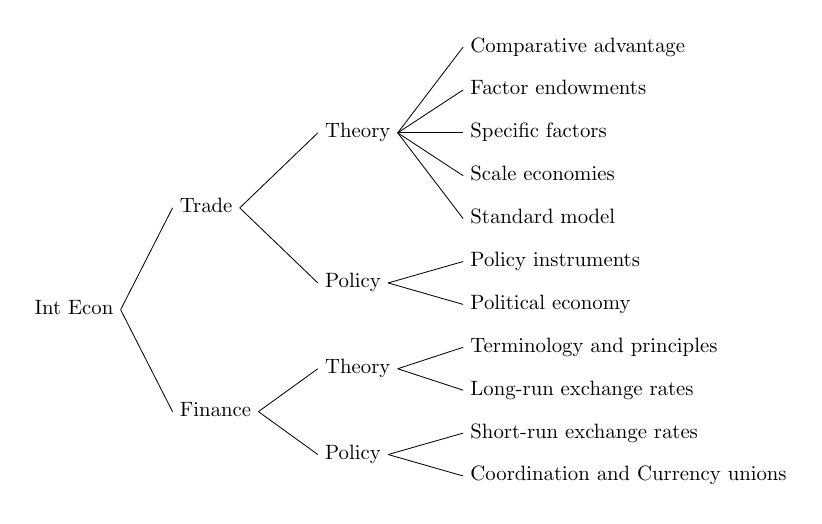
\begin{tikzpicture}
\tikzset{scale=0.75,grow'=right,level distance=70pt}
\tikzset{execute at begin node=\strut}
\tikzset{every tree node/.style={anchor=base west}}

\Tree   [.Int\ Econ                     [.Trade     [.Theory    [.Comparative\ advantage ]
                                                                [.Factor\ endowments ]
                                                                [.Specific\ factors ]
                                                                [.Scale\ economies ]
                                                                [.Standard\ model ] ]
                                                    [.Policy    [.Policy\ instruments ]
                                                                [.Political\ economy ] ] ]
                                        [.Finance   [.Theory    [.Terminology\ and\ principles ]
                                                                [.Long-run\ exchange\ rates ] ]
                                                    [.Policy    [.Short-run\ exchange\ rates ]
                                                                [.Coordination\ and\ Currency\ unions ] ] ] ]
\end{tikzpicture}
\end{frame}





\end{document}
